% !TEX root = ../../numb3rs.tex
\newpage
\subsection{205: Assassin\label{205}}

While attempting to bring into someone into custody for making fake IDs, Agents Don Epps and Megan Reeves discover a notebook containing pages and pages of blocks of letters in code. Handing off the notebook to Charlie, he quickly identifies the content as codes pertaining to ``assassination,'' ``target'', and ``secret.'' He broke the assassin's code, thus giving the FBI enough warning to prevent the murder of a young Colombian political exile. \\

%%%%%%%%%%
\temph{What is Cryptography?}
%%%%%%%%%%

Cryptography is one of the oldest areas of mathematics for this very reason. For as long as people have communicated, there are messages that we would like \emph{some} people to have and not others. Even outside of wartime - when having your privileged information \emph{remain} privileged could mean the lives of hundreds or of thousands -- there are numerous areas where being able to transmit information and have it remain secure is vital. For example, for any sort of large scale commerce, the ability to transfer and protect an increasingly digital set of assets is vital -- and would you ever be willing to pay for something online with a credit card if your card number wasn't being encrypted before being sent? \\

Historically, cryptography is the ``art of secret writing.'' Given a message, we have both a method of \emph{encoding} it into a (theoretically) unintelligible new message, along with a method of \emph{decoding} these unintelligible messages back into plain text. Collectively, this pair of encoding and decoding procedures is called a ``cypher.'' Some of the oldest cyphers are \bref{transposition cyphers}{https://en.wikipedia.org/wiki/Transposition_cipher} and \bref{substitution cyphers}{https://en.wikipedia.org/wiki/Substitution_cipher}. \\

\fbox{\begin{minipage}{43em}
\begin{center} \large \dotuline{Tangent}  \\ \end{center}
Caesar Cyphers: Substitution cyphers, or cyphers where encryption and decryption involve the replacement of letters (either singly, in pairs, or in groups) with other letters or symbols, are a classic and familiar type of code. A specific \emph{type} of substitution cypher was even a traditional favorite of Julius Caesar himself! \bref{Caesar cyphers}{https://en.wikipedia.org/wiki/Caesar_cipher}, in general, refer to substitution cyphers where you replace the letter A by some letter, say perhaps G. Next B is replaced by H, C by I, D by J, and so on -- sliding each letter down a fixed number of spaces from the first letter. \\

Caesar is said to have favored this type of code with a shift of three letters. Admittedly, now it seems silly, but when the majority of your contemporaries are unlikely to be able to read - much less consider intercepted gibberish vital -- it isn't such a bad idea!
\end{minipage}} \vspace{0.2cm}

\fbox{\begin{minipage}{43em}
\begin{center} \large \dotuline{Activity 1}  \\ \end{center}
 Assume the following is a Caesar cypher. If R goes to N, decode the secret message! 
	\[
	\text{E YWIA E OWS E YRJMQANAZ}
	\]
The following is a Caesar cypher. Try to decode this without knowing beforehand how many letters to move forward. \\
	\[
	\text{HWD MFATP FSI QJY XQNU YMJ ITLX TK BFW!}
	\]
Here's one more (non-Caesar) cypher for warm-up. Enjoy! 
	\[
	\text{EM TO KEERG SAW TI, TRAP NWO YM ROF, TUB}
	\]
\end{minipage}} \vspace{0.2cm}




\fbox{\begin{minipage}{43em}
\begin{center} \large \dotuline{Tangent}  \\ \end{center}
RSA Algorithm and Public Key Cryptography: So far, it's been a trade-off between being too easy to decode something even without the key (basic substitution cyphers, especially transposition cyphers) or too hard (or impossible) to encode something without already knowing the key. The invention of ``public key'' cryptography is an attempt to have the best of both worlds -- we'd like to have anyone be able to encode data (with or without the key), but still have our encrypted data remain secure. One way it is done is having a distinction between public and private keys. A public key is sufficient to encode data, while the private key is kept secure and used to decode data. \\

Perhaps the most famous of the public key systems is RSA, named for Ron Rivest, Adi Shamir and Leonard Adleman, which works basically according to the following:
\begin{enumerate}[1.]
\item We choose distinct large primes $p$ and $q$. When we say large, we mean these primes are on the order of 512 to 1024 bits each.
\item We compute their product, $n=pq$.
\item We compute the totient of $n$, written $\phi(n)=(p-1)(q-1)$.
\item We choose some integer $e$, which is the public key or public exponent. This needs to be relatively prime to our modulus $n$, and typically, it will be in the thousands.
\item We choose some other integer $d$ such that $d\cdot e$ is congruent to 1 modulo our totient function of $n$, i.e. we have that $d \cdot e \equiv 1 \mod \phi(n)$ or rather, $d \cdot e= 1 + m\phi(n)$, where $m$ is some integer. This key is the private key or private exponent.
\end{enumerate}

Now we have our private and public key. How do we encode or decode messages? 
	\begin{figure}[H]
	   \centering
	   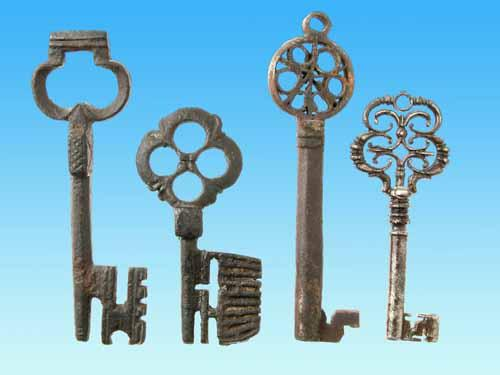
\includegraphics[width=0.38\textwidth]{season2/205/images/keys.jpg} 
	\end{figure}
\begin{itemize}
\item Well, encoding is easy. I turn message $M$ into an appropriate number $m$, then compute $m^e \mod n$.
\item Knowing $d$, we can quickly recover the original message from our received message $m'$ by the following: $(m')^d \mod n=m$
\end{itemize}

This follows pretty readily from the way we chose $e$ and $d$, as we have that in Step 5 we selected $e \cdot d$ to be congruent to 1 mod $(p-1)(q-1)$, that $(m')^d \mod n =(m^e)^d \mod n = m^{ed}$ and $ed \equiv 1 \mod (p-1)^d$ and $ed \equiv 1 \mod q-1$. From Fermat's little theorem, this gives us that $m^{ed} \equiv m \mod p$ and $m^{ed} \equiv m \mod q$ and hence, that $m^{ed} \equiv m \mod n$. So long as large numbers are hard to factor -- namely, our number n, on the order of 1024 to 2048 bits long -- it is easy to encrypt with the public key and easy to decrypt with the public and private key, but computationally infeasible to decrypt without the private key.
\end{minipage}} \vspace{0.2cm}



\fbox{\begin{minipage}{43em}
\begin{center} \large \dotuline{Activity 2}  \\ \end{center}
Practicing Encoding/Decoding Using RSA: First off, we're going to practice using a specific $p$ and $q$, let's say $p=193$ and $q=131$. 
\begin{enumerate}[1.]
\item Calculate $n$ and the totient of $n$. Factor totient of $n$. (Hint: There should be four distinct primes!)
\item Let $e_1=17$ and $e_2=23$. Check which of $d_1=9767$ and $d_2=5873$ satisfies the conditions we'd need for a private key with either of them. What does $e\cdot d$ equal modulo 24960 for each possible pair of e's and d's?
\item Encrypt the ``message'' 2 into its encoded form with $e_1$ and whatever $d$ matched. Remember, you're working modulo $n$! Now imagine trying to take this number and decrypt it by hand. Or by hand, without even knowing what $d$ was.
\item If you want to try practicing with higher numbers, check out \bref{this}{http://demonstrations.wolfram.com/RSAEncryptionAndDecryption/} or \bref{this}{http://demonstrations.wolfram.com/StrongRSACryptosystem/}. You can see what sorts of calculations this would run into with genuine public keys!
\end{enumerate}
\end{minipage}} \vspace{0.2cm}

